\section{Calculating Potential and Electric Field of Parallel Plate Capacitor}
\label{sec:parallel_plate_capacitor}

Next the program to solve Laplace's equation in two dimensions is applied to two equipotential plates, i.e. a parallel plate capacitor. The potential and electric fields are plotted in Figures \ref{subfig:capacitor_surf_big} and \ref{subfig:capacitor_vector_big}. Figure \ref{subfig:capacitor_surf_big} shows that between the positive plate on the left and the negative plate on the right, the surface of the potential field has a constant gradient. Figure \ref{subfig:capacitor_vector_big} also demonstrates clearly that between the two plates, the electric field is linear and constant, as is expected. Around the ends of the plates it can also be seen that the infinite plate approximation breaks down and the field lines curve away from the region of constant electric field strength.

\begin{figure}
    \centering
    \subfloat[Surface plot.]{
        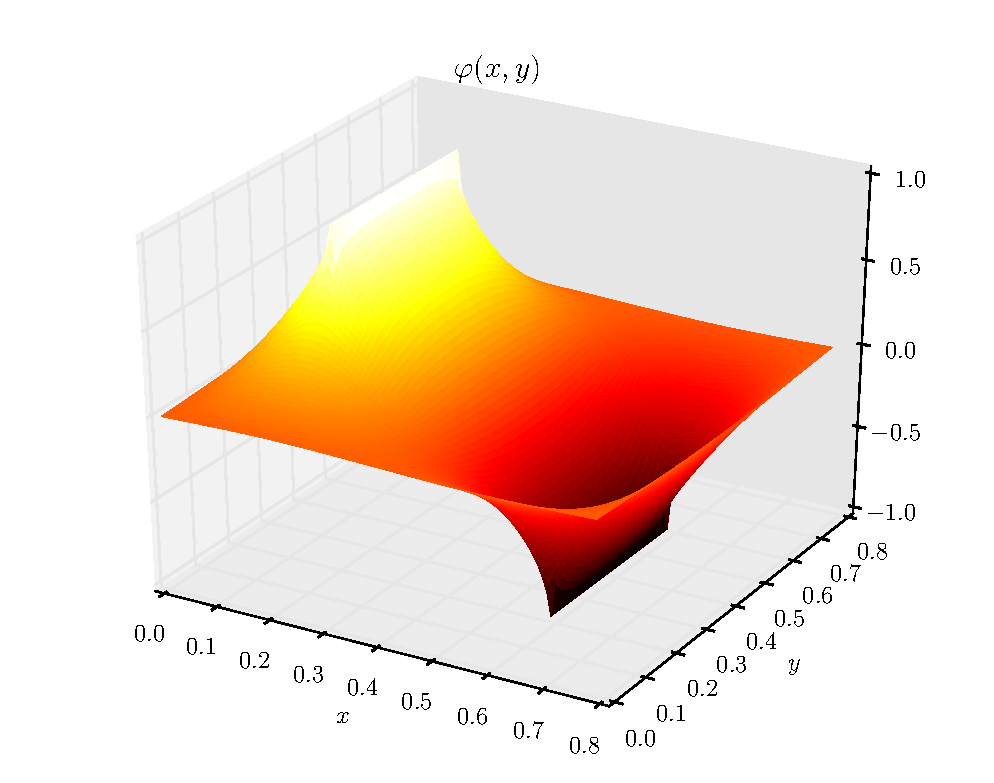
\includegraphics[width=0.5\linewidth]{graphs/examples/capacitor_surf}
        \label{subfig:capacitor_surf_big}
    }
    \subfloat[Electric field lines plot.]{
        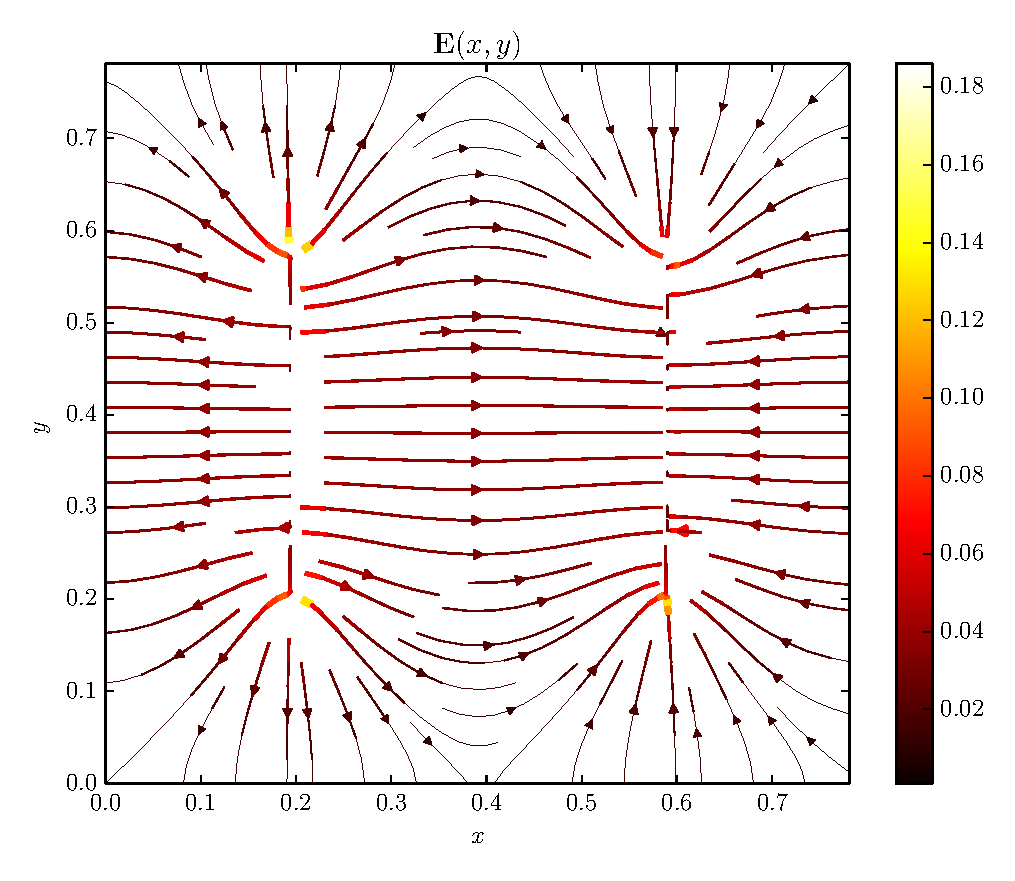
\includegraphics[width=0.5\linewidth]{graphs/examples/capacitor_vector}
        \label{subfig:capacitor_vector_big}
    }
    \caption{Surface plot of the solution to Laplace's equation in and around a parallel plate capacitor.}
    \label{fig:capacitor_big}
\end{figure}

\subsection{Infinite Plate Solution}
\label{subsec:infinite_plate_solution}

When the distance between the plates, $d$, is large compared to the width of the capacitor plates, $a$, the capacitor looks like a dipole, as shown in Figures \ref{subfig:small_capacitor_contour} and \ref{subfig:small_capacitor_magnitude}. As the plates are brought closer together and the width increases, i.e. the ratio $\frac{a}{d}$ increases, the solution looks more and more like the infinite plate solution, namely $E=0$ outside the capacitor and $E = \frac{V}{d}$ inside the capacitor. Figures \ref{subfig:long_capacitor_contour} and \ref{subfig:long_capacitor_magnitude} shows a wide parallel plate capacitor where the plates are very close together. As can clearly be seen, both the potential surface and the electric field lines corroborate the infinite plate solution inside the capacitor, where the potential surface is an inclined plane and the electric field lines are straight lines from positive plate to negative plate. Figure \ref{subfig:long_capacitor_magnitude} shows that when $\frac{a}{d}$ is large, the magnitude of the field outside the capacitor goes almost completely to zero. Quantitatively, if a potential difference of \SI{2}{V} is maintained between two capacitor plates 4 nodes apart ($d=4$ nodes) with width 98 nodes ($a=98$ nodes) with grid density 100 by 100, as shown in Figures \ref{subfig:long_capacitor_contour} and \ref{subfig:long_capacitor_magnitude}, then the average electric field strength outside the plates is \SI{0.02}{\volt} and inside the plates is \SI{0.49}{\volt}. As $E=\frac{V}{d}=1/2$, this is extremely close to the infinite plate solution. The slight offset from this infinite plate solution is due to the edges of the plates having slightly lower electric field strength than in between the plates, as can be seen in Figure \ref{subfig:long_capacitor_magnitude}. The calculated solution to the Laplace equation for a parallel plate capacitor thus approximates the infinite plate solution extremely well when the ratio of the plate width to separation is large.

\begin{figure}
    \centering
    \subfloat[Small $\frac{a}{d}$.]{
        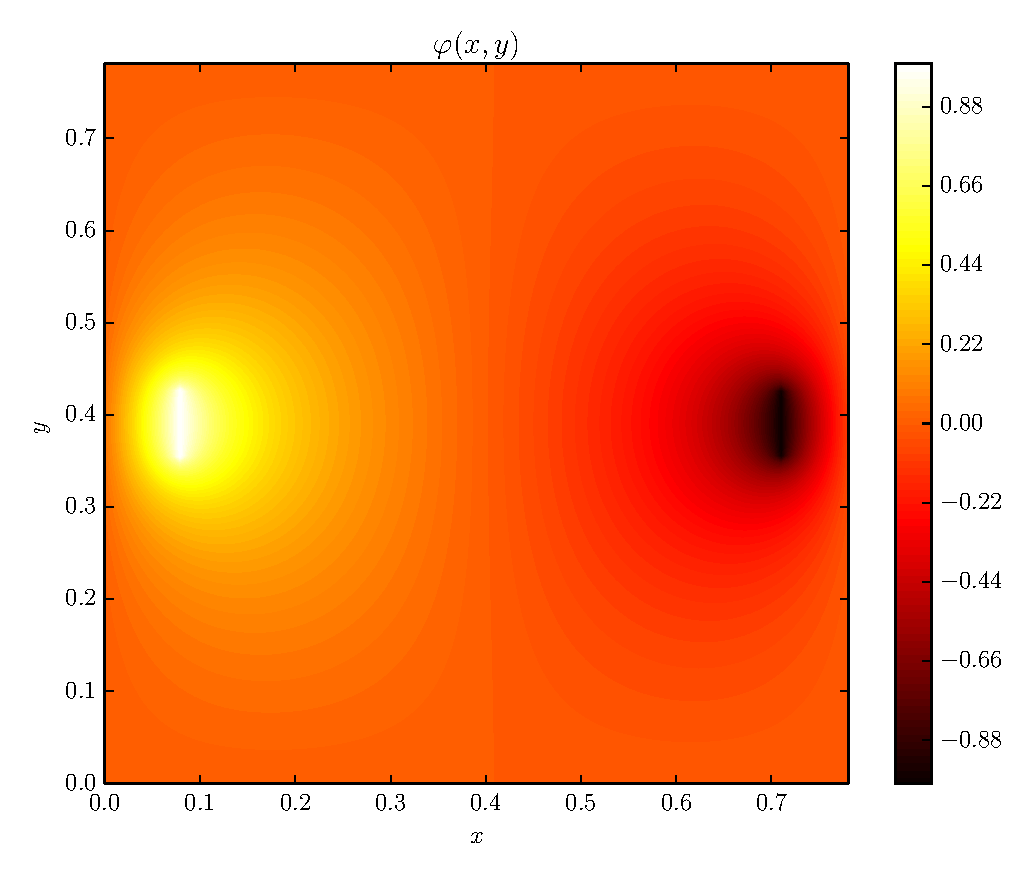
\includegraphics[width=0.5\linewidth]{graphs/capacitor/small_capacitor_contour}
        \label{subfig:small_capacitor_contour}
    }
    \subfloat[Large $\frac{a}{d}$.]{
        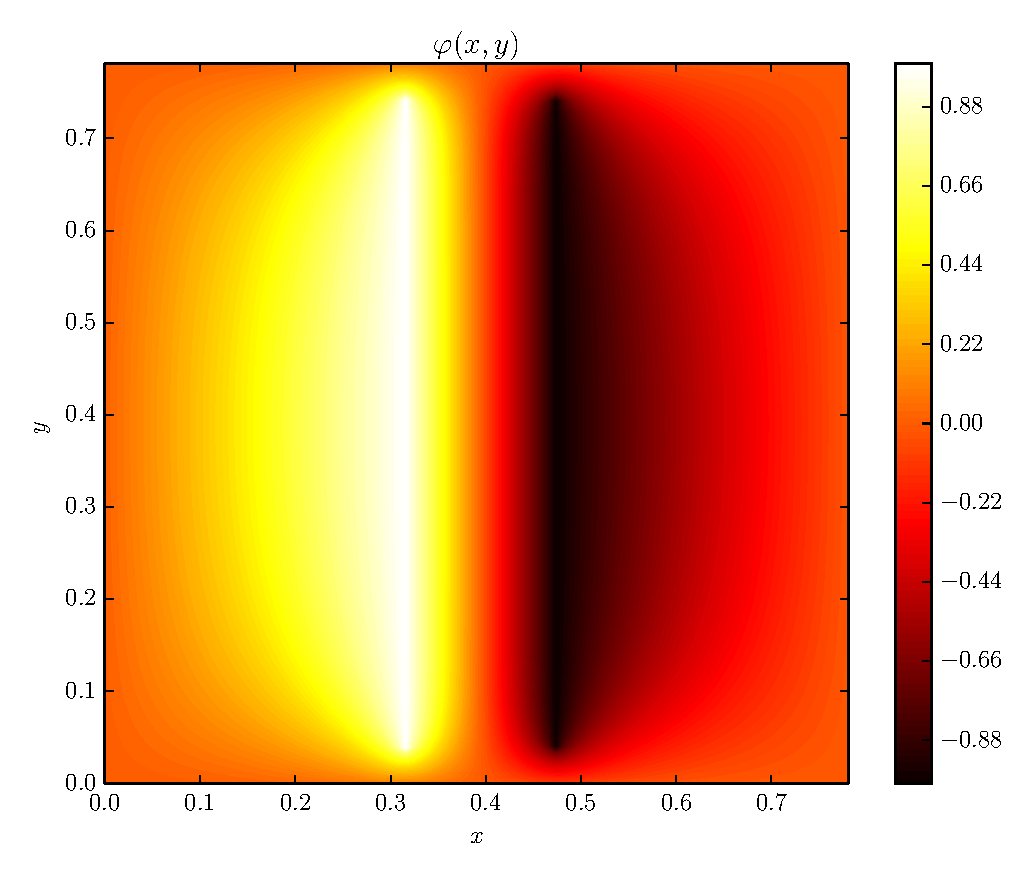
\includegraphics[width=0.5\linewidth]{graphs/capacitor/long_capacitor_contour}
        \label{subfig:long_capacitor_contour}
    }
    \caption{The potential field contours around a parallel plate capacitor for small and large $\frac{a}{d}$.}
    \label{fig:capacitor_sizes_contour}
\end{figure}

\begin{figure}
    \centering
    \subfloat[Small $\frac{a}{d}$.]{
        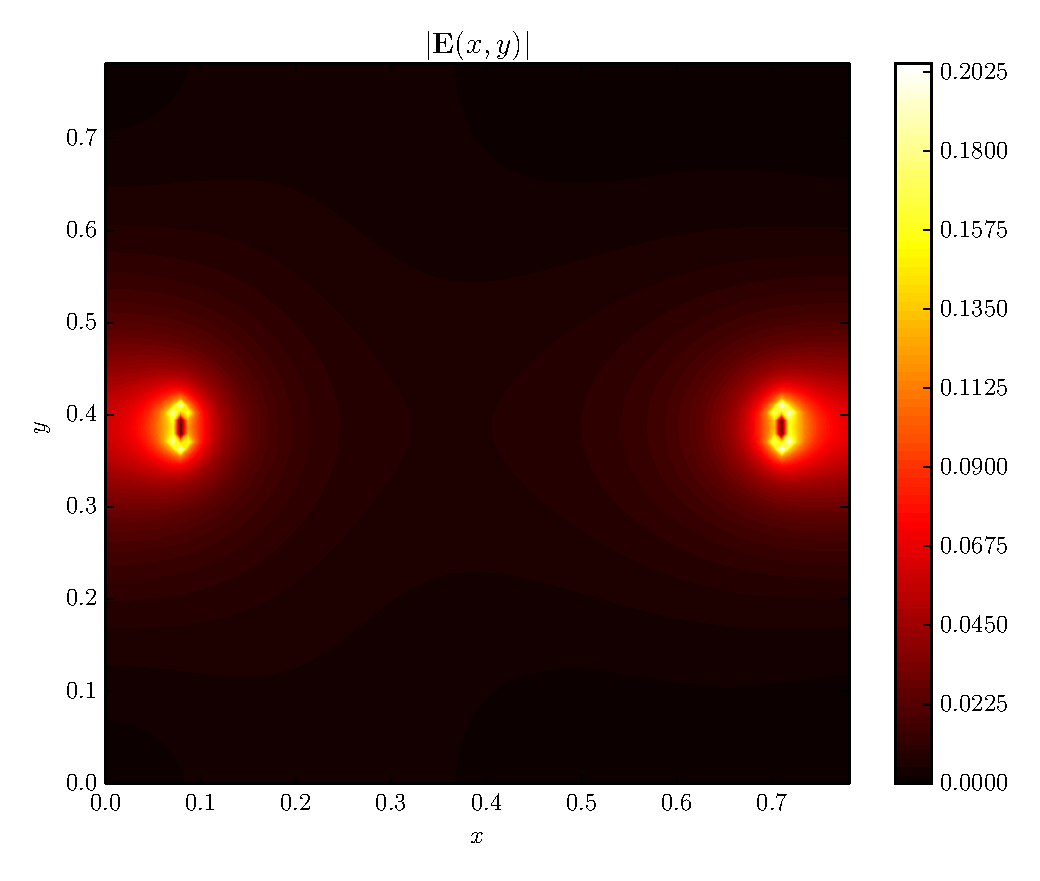
\includegraphics[width=0.5\linewidth]{graphs/capacitor/small_capacitor_magnitude}
        \label{subfig:small_capacitor_magnitude}
    }
    \subfloat[Large $\frac{a}{d}$.]{
        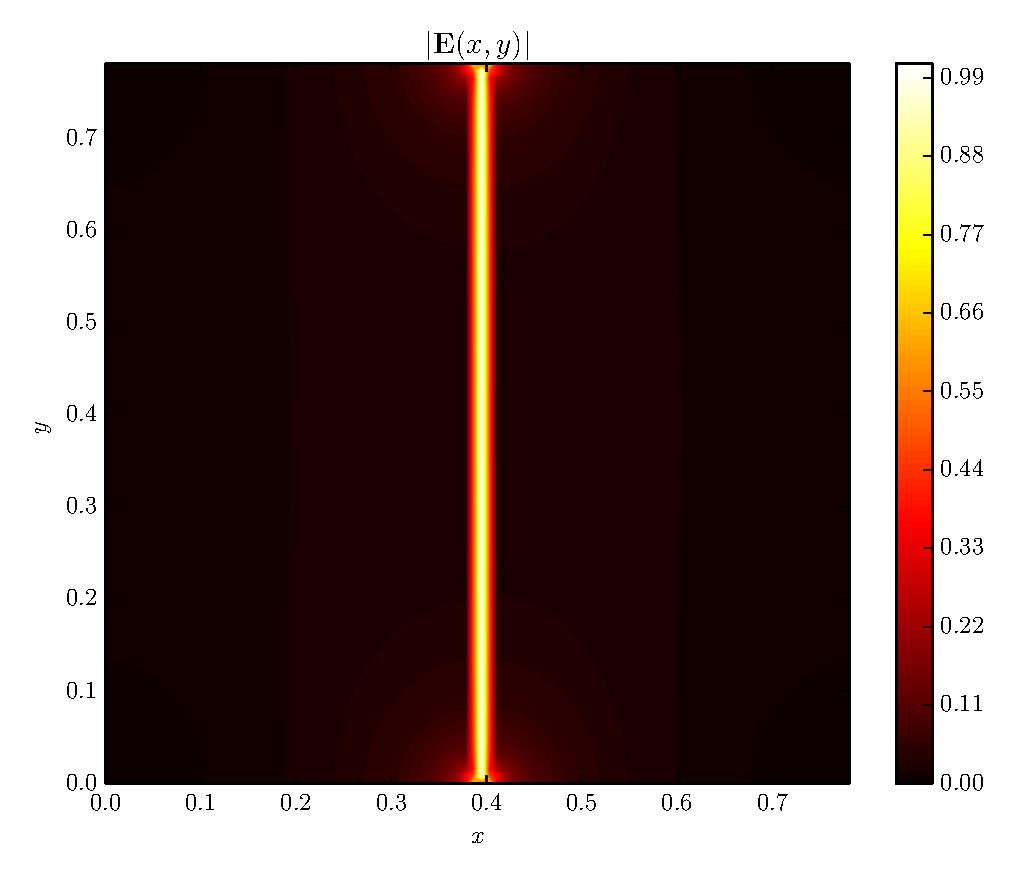
\includegraphics[width=0.5\linewidth]{graphs/capacitor/long_capacitor_magnitude}
        \label{subfig:long_capacitor_magnitude}
    }
    \caption{The magnitude of the electric field contours around a parallel plate capacitor for small and large $\frac{a}{d}$.}
    \label{fig:capacitor_sizes_magnitude}
\end{figure}
